\section{Cos'\`{e} \LaTeX?}
\frame{\transfade\centering
\LaTeX{} \only<2>{(/\textipa{"la:tEx}/,[\textipa{"latek}]; dal greco \begin{otherlanguage}{greek}τέχνη\end{otherlanguage})}\only<3->{è un linguaggio di markup.}
\only<4->{\\~\\Descrivere il documento}
\only<5->{\begin{figure}
  \captionsetup[subfigure]{labelformat=empty}
  \centering
  \begin{subfigure}[b]{0.4\textwidth}
      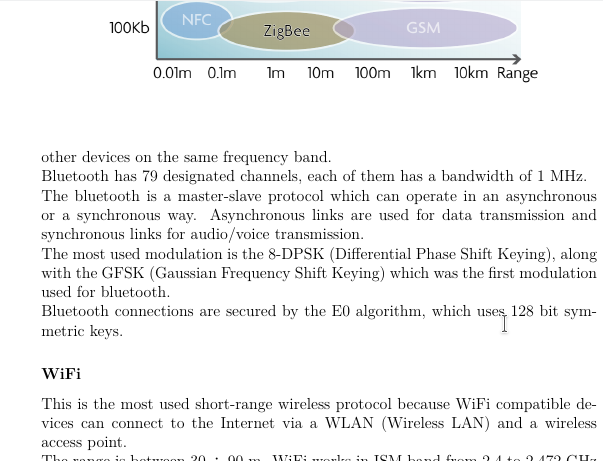
\includegraphics[width=\textwidth]{img/writer}
      \caption{Writer}
  \end{subfigure}~
  \visible<6->{\begin{subfigure}[b]{0.4\textwidth}
      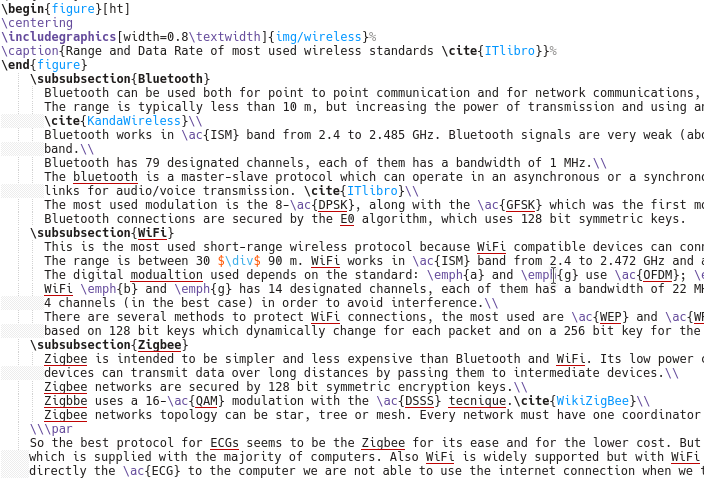
\includegraphics[width=\textwidth]{img/latex_source}
      \caption{Latex}
  \end{subfigure}}
\end{figure}}
}

\frame{\transfade\centering
\frametitle{I vantaggi di \LaTeX}
\begin{itemize}
\item<2-> i documenti hanno un'impaginazione perfetta e risultano piacevoli alla lettura
\item<3-> con un po' di esercizio di possono comporre formule matematiche, schemi a blocchi, circuiti,\dots{} semplicemente
\item<4-> la formattazione non subirà mai modifiche drastiche e risulterà uniforme
\end{itemize}
}

\frame{\transfade\centering
\frametitle{Cosa si può fare con \LaTeX?}
\only<1>{
  \begin{columns}\begin{column}{0.4\textwidth}\centering
  Articoli, Relazioni, Libri, Lettere,~\dots
  \end{column}\begin{column}{0.6\textwidth}
  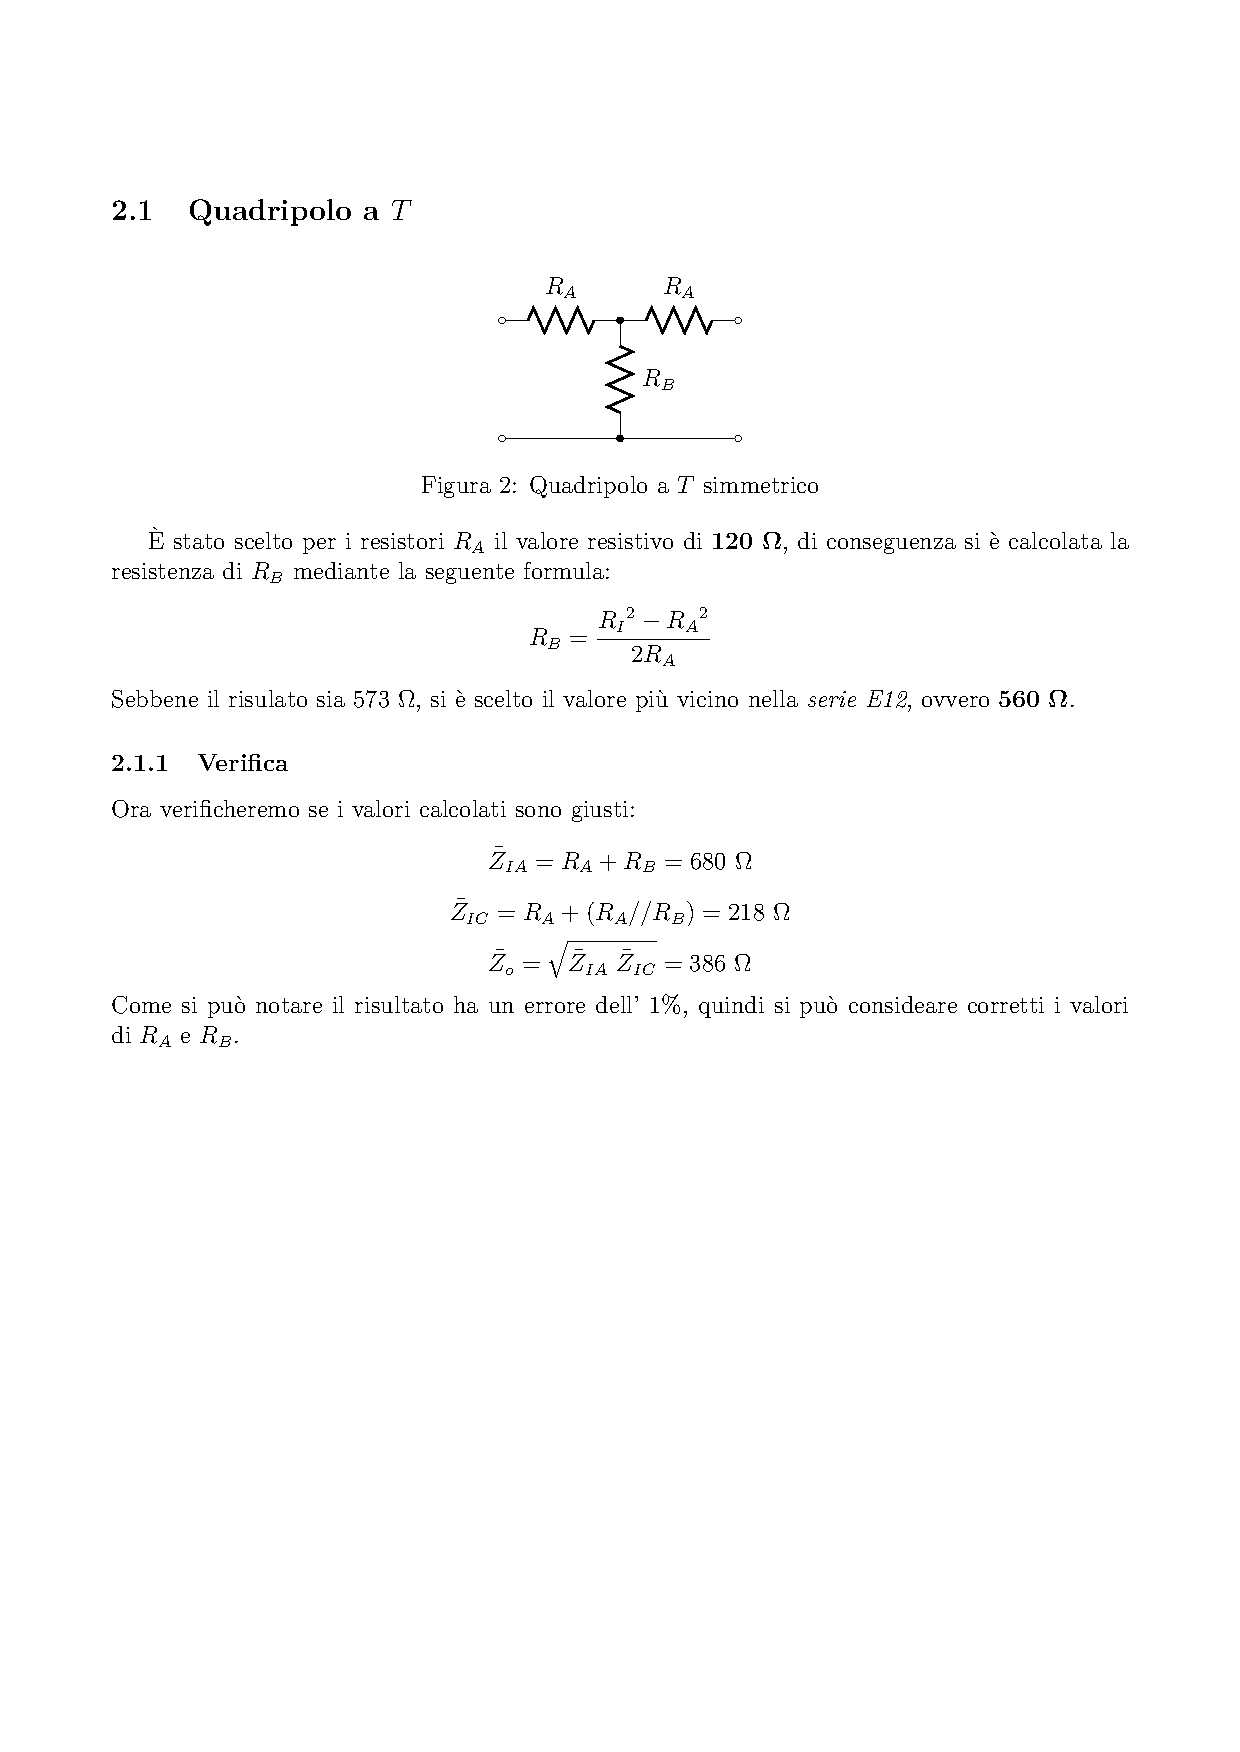
\includegraphics[height=0.8\textheight]{img/relazione}
  \end{column}\end{columns}
}
\only<2>{
  Circuiti, Schemi, Tabelle, Grafici,~\dots\\
  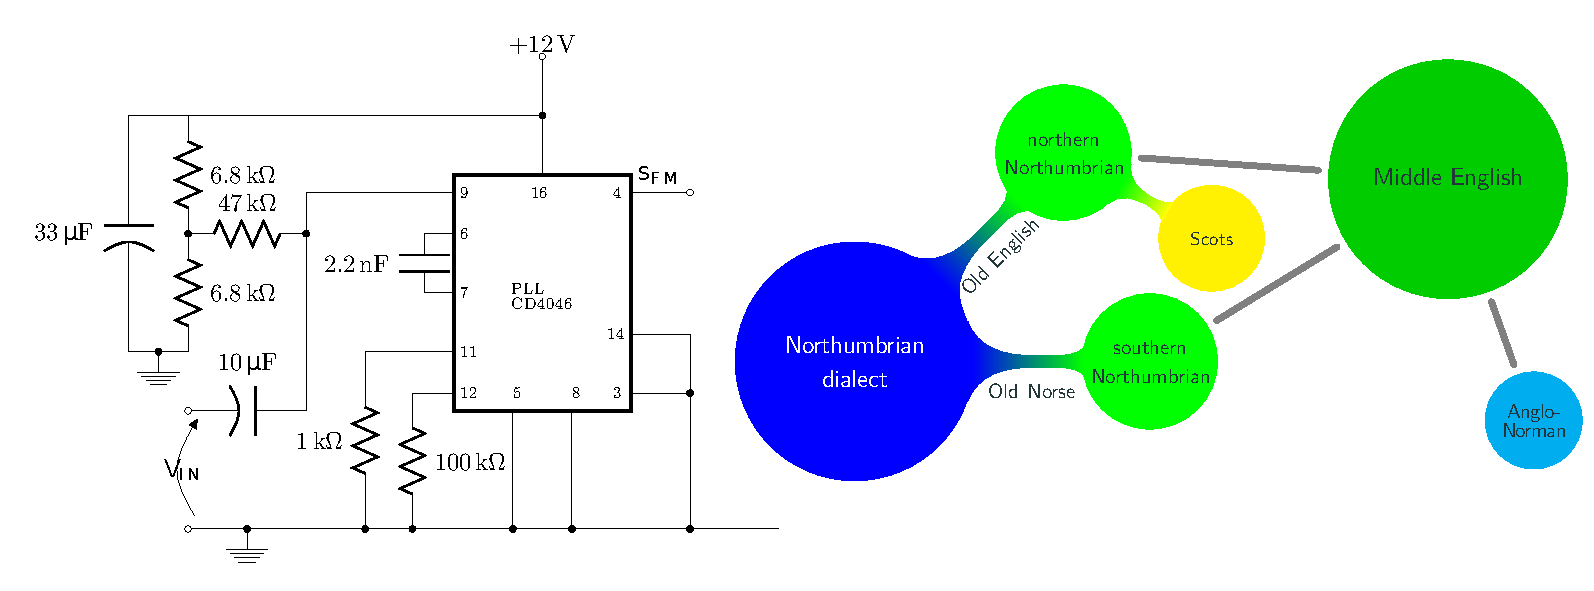
\includegraphics[width=0.9\textwidth]{img/schemi}
}
\only<3>{
  Formule chimiche\\
  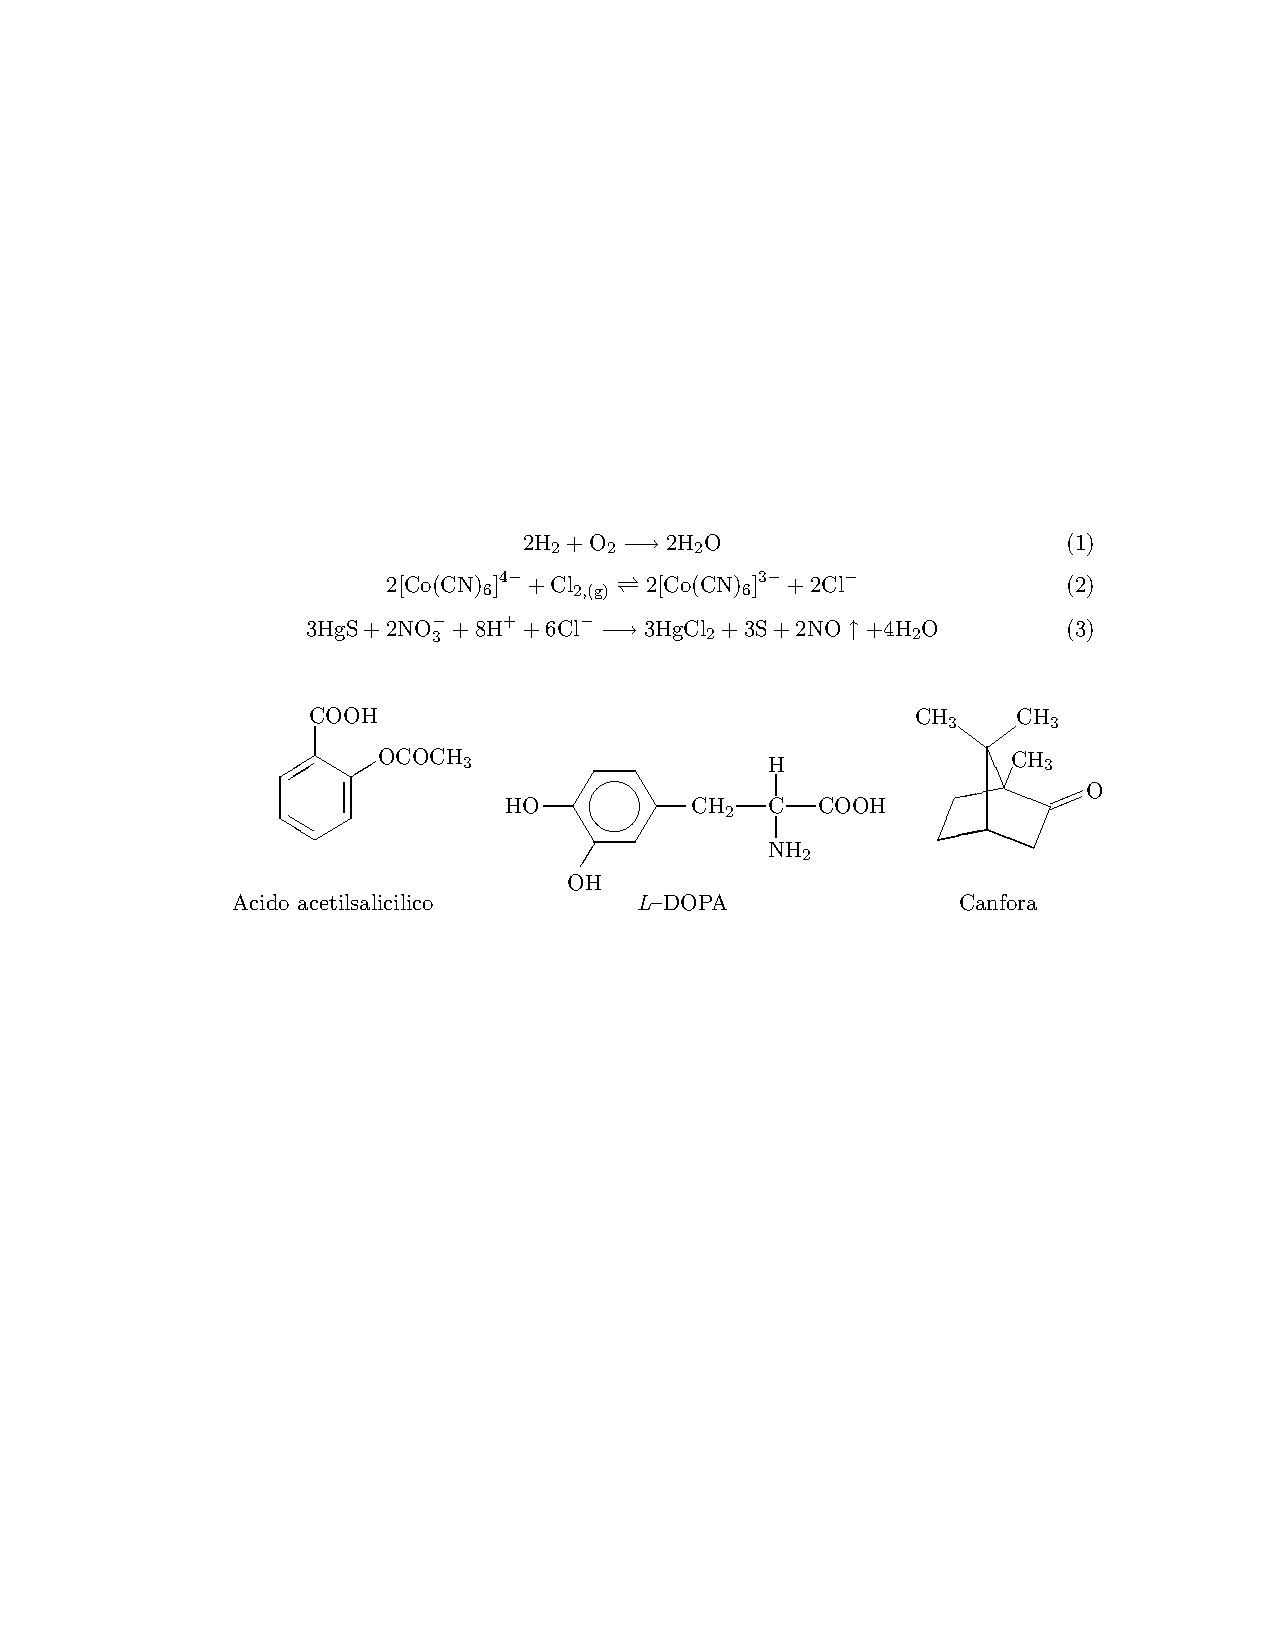
\includegraphics[width=0.9\textwidth]{img/chimica}
}
\only<4>{
  Accordi, Spartiti,~\dots\\
  \begin{figure}
    \captionsetup[subfigure]{labelformat=empty}
    \centering
    \begin{subfigure}[b]{0.4\textwidth}
        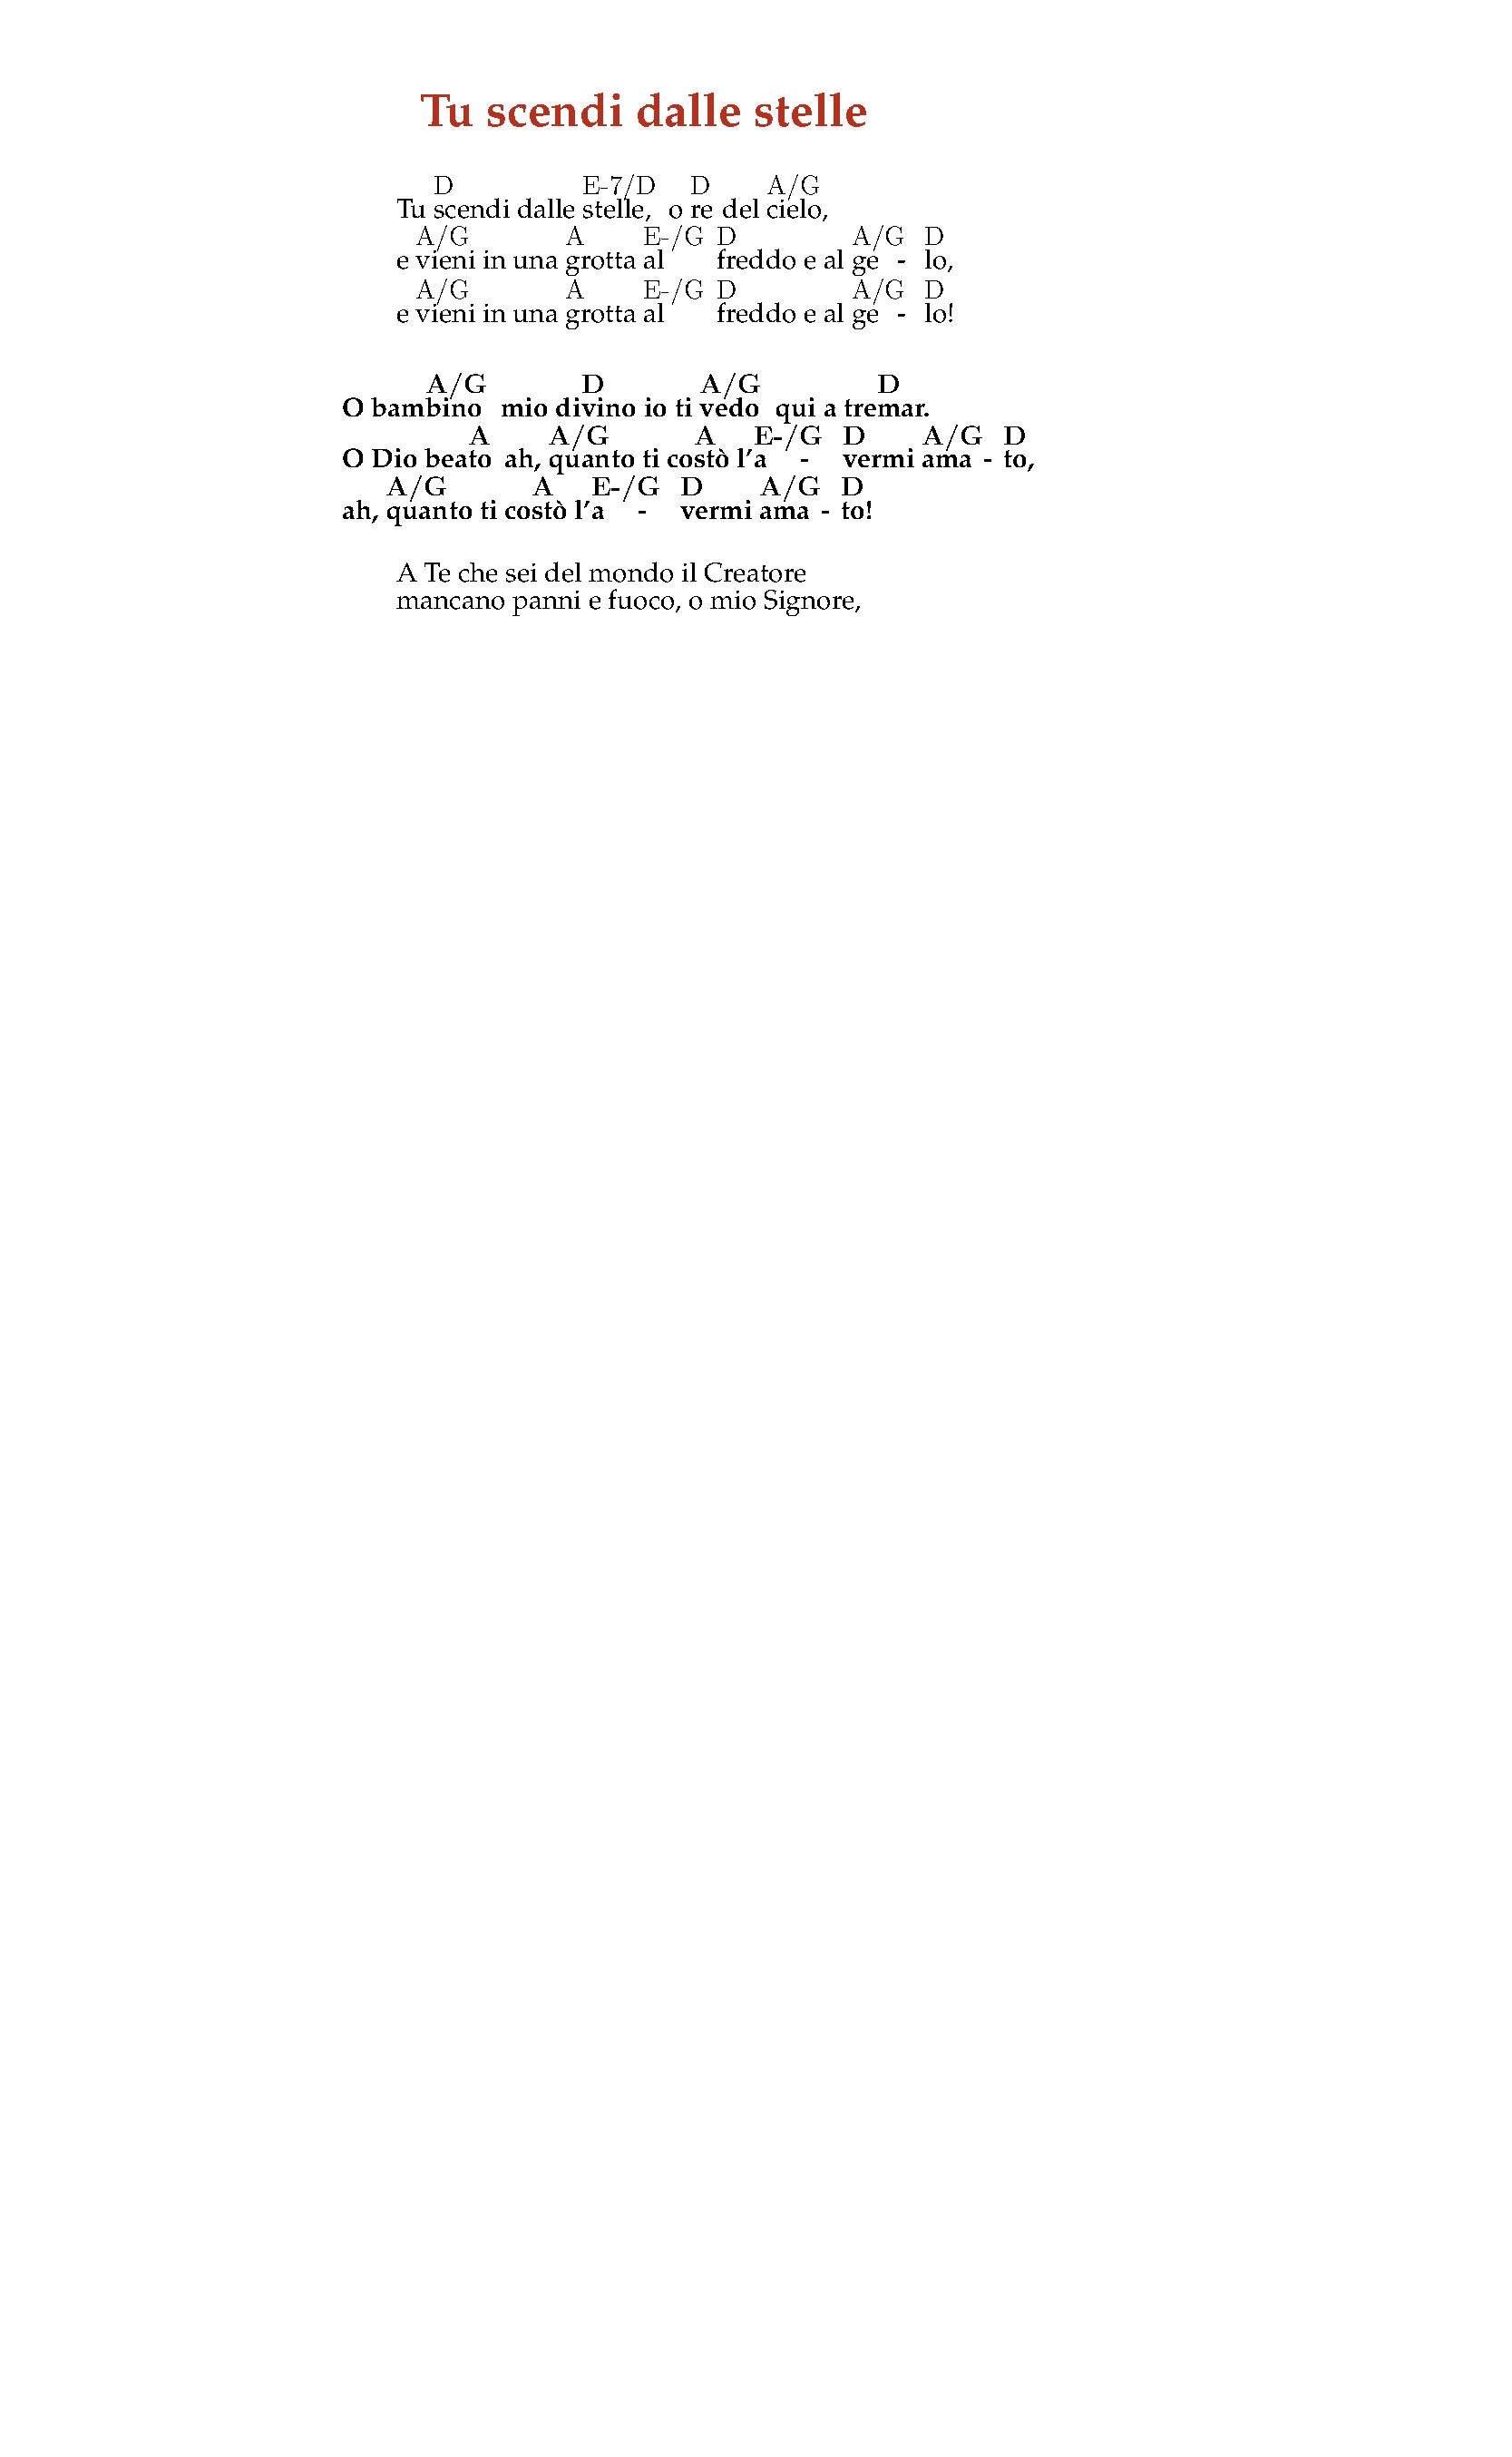
\includegraphics[width=\textwidth]{img/accordi}
    \end{subfigure}~
    \begin{subfigure}[b]{0.6\textwidth}
        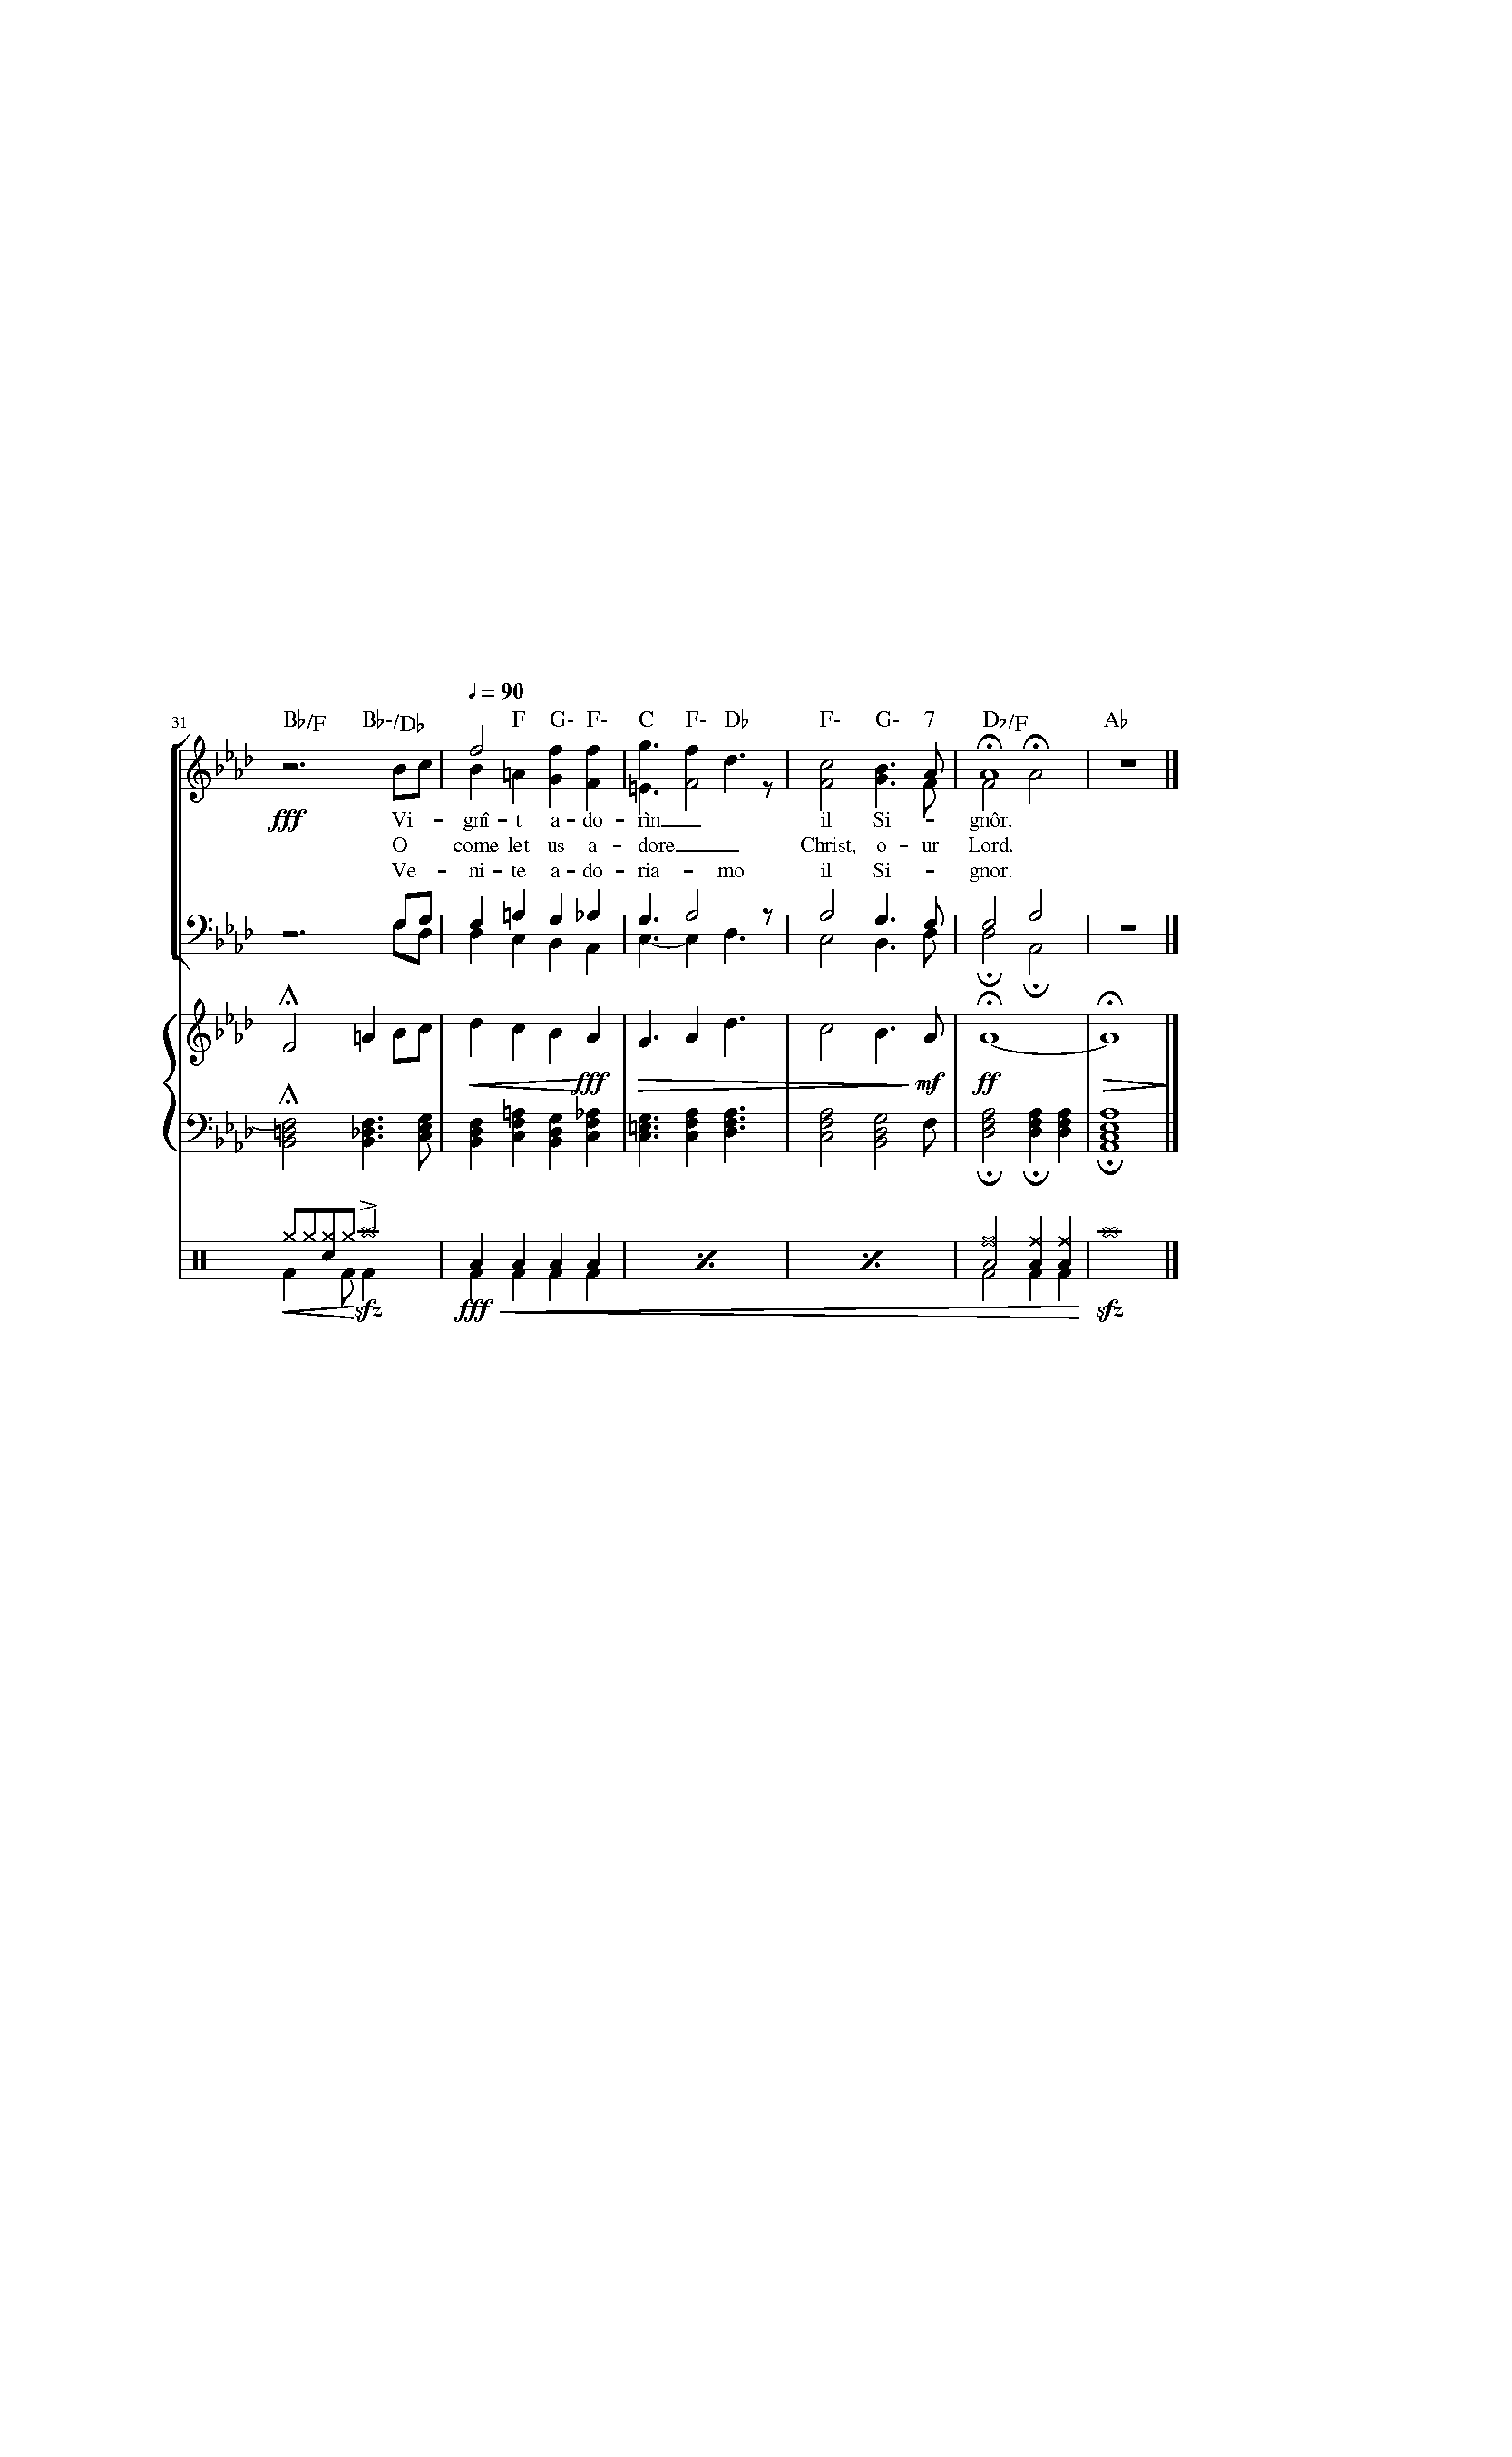
\includegraphics[width=\textwidth]{img/spartiti}
    \end{subfigure}
  \end{figure}
}
\only<5>{
  Presentazioni\\~\\
  \fbox{
\includegraphics[width=0.7\textwidth,page=1]{img/presentazione}}
}
\only<6>{
  Scrivere facilmente con più alfabeti\\~\\
  
\includegraphics[width=\textwidth,page=1]{img/alfabeti}
}
}

\frame{\transfade\centering
\frametitle{Come si utilizza \LaTeX?}
\begin{itemize}
  \item<2->{Editor di testo + linea di comando}
  \item<3->{Editor avanzato (es: Miktex)}
\end{itemize}
}